
\section{Compression of data}

This section will investigate the theory behind data compression, as well as trying to find compression techniques that could be used in the application. This study was requested by Thales.
\newline

Source coding, better known as data compression, is a way of reducing resource usage by compressing data. It performed on the data source before storing or transmitting the data. By encoding the data using fewer bits than the original representation the size of the data file decreases.

\begin{figure}[h!]
\begin{center}
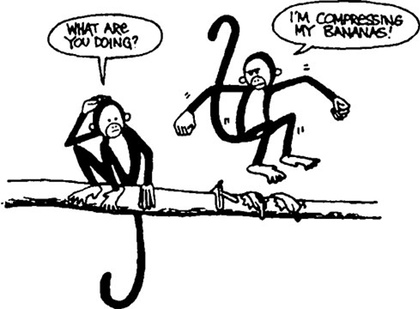
\includegraphics[scale=0.5]{compressionmonkeys}
\caption{Compression in practice \cite{bib:compressionImage}}
\end{center}
\end{figure}

\subsection{Benefits}
Compression is mainly used to reduce data storage space and transmission capacity. For the XOXOmail application both these features are important reasons to use data compression, but the most important is the one evolving transmission capacity. Since the users of the XOXOmail should be able to send pictures and videos as well as text, it is crucial to make the attachments as small as possible so that sending of a message with such attachments is possible, also in networks with poor bandwidth.

\subsection{Disadvantages}
Because that the data is compressed when receiving it, it must be decoded before use. This decoding is often resource demanding. Decoding of text and images are not very expensive and is done pretty fast.  When it comes to compressing and decompressing of video it is a quite different story. To encode a video without losing data is a time consuming task which requires expensive hardware. If the process is to slow, it will not be possible to watch the movie while it is being decoded. It is important to note that the result of decoding a compressed video may or may not give a different result thant the original data. This is dependent of the compression method used.

\pagebreak

\subsection{Data compression approaches}
There are two main ways to perform data compression. The two types are lossy and lossless data compression \cite{bib:dataCompression}. First we will describe lossy data compression as well as techniques for this method, then continue to do the same for lossless data compression.

\subsubsection{Lossy data compression}
Lossy compression means that data is lost during the compression procedure. When encoding the image, you do not get the original image out, because data is lost during the process. The purpose is to decrease the amount of data that must be sent or handled. Often the data, especially multimedia data, can be useful even though some of the data is lost, e.g. an image that will become coarser but still be very much like the full version. The compression algorithms often use well known properties of the human eye to remove details we cannot see. This makes it very hard to see the difference between a compressed and and uncompressed image. A well known usage of lossy compression is in streaming.  \cite{bib:lossyCompression}

\paragraph{Lossy compression techniques for images} \hfill \newline

Lossy copression of images is done by using various algorithms that removes information from the original file. A range of different alternatives exist here, and the results are varying. Some of the algorithms do compression with different ratios, and still uses the same time to compress. Examples of lossy compression standards for images are JPEG and PGF  \cite{bib:JPEG} \cite{bib:PGF}.  

\paragraph{Lossy compression techniques for video} \hfill \newline

Compression of video can be divided into two main groups: Inter and intra frame. The difference is in how we find out how we can compress. In inter frame encoding we look at a given set of frames in a special order and compress based on similarities between them, while we in intra frame encoding only look at one image at the time, which will be the same as image compression.\cite{bib:DV} \cite{bib:DV} \cite{bib:Dirac} \cite{bib:VC-1} 


\paragraph{Lossy compression techniques for audio}  \hfill \newline
Lossless compression of audio is done by removing frequencies not audible for the human ear. This reduces the data size a lot. We often compress audio more than this to make the audio files so small that they can fit without problems on portable devices like mobile phones and laptops. The most common file formats here are MP3, AAC and WMA.\cite{bib:MP3} \cite{bib:AAC} \cite{bib:WMA}

\subsubsection{Lossless data compression}
There will come a point where lossy compression will have made the original data useless. Although the human eyes and ears may not catch small degradations of images and sounds, the decreased quality eventually will be apparent.
\newline
\newline
To have lossless compression means that the reconstruction of the compressed data is identical to the original data. A well-known example is the ZIP file format. Lossless compression is used when it is important that the original and decompressed data is identical, e.g. text or source code. The common way of doing lossless compression is to first generate a statistical model for the input data and secondly use this model to map input data to bit sequences. There are two ways of constructing statistical models. The first is to use static models, where data is analyzed and a model constructed, then the model is stored with the compressed data. This method is simple and modular, but the model can be expensive to store and the method may not perform well on files with heterogeneous data, as all data will have the same mode. The second method is to use an adaptive model. Here the model is dynamically updated as the data is compressed. The model is trivial at first but improves rapidly.
\newline
\newline
The most used encoding algorithms for producing bit sequences are Huffman coding and arithmetic coding. There are many special-purpose compression algorithms for e.g. images, text and video. In addition, there are many general-purpose lossless compression algorithms that may be used on any type of data. The problem arises when the input data is on another form than the algorithms were originally designed to compress.
A list of some common techniques and formats for lossless encodings will follow. \cite{bib:losslessCompression}


\paragraph{Lossless compression tecniques for text} \hfill \newline

Lossless compression of text is tricky. It has to have good performance and guarantee that the result of converting it back to the original data gives the correct result. Context tree weighting and LZ77 are examples of compression algorithms often used  \cite{bib:contextTreeWeightingResearch}. It is often advantageous to transform data to a format that compression algorithms will run better on. An example of such an algorithm is the Burrows-Wheeler transform \cite{bib:burrowsWheelerTransform}. 

\paragraph{Lossless compression tecniques for images}  \hfill \newline
When we are doing lossless compression of images, we must find data in the image that is redundant and find a better way of representing it. This is why lossless compression of images works best on images with large areas of identical color. Examples of image formats often used are GIF and PNG. \cite{bib:GIF} \cite{bib:gifsicle} \cite{bib:PNG}

\paragraph{Lossless compression tecniques for video}  \hfill \newline
The same principle holds for lossless video compression as for image compression; a lot of area with similar coloring is necessary for good performance. If a inter frame compression algorithm is used, we will get much better compression ratio compared to intra frame, but it requires a lot of processing power. Examples of algorithms are CorePNG and Animation Codec \cite{bib:corePNG} \cite{bib:animationcodec}


\paragraph{Lossless compression techniques for sound}
The most common formats used for lossless compression of sound is FLAC and MPEG-4 SLS. They both are able to compress the data with 50-60\% . The biggest problem of compressing using these standards, is that they are often not supported on portable devices.  \cite{bib:FLAC}


\subsection{Discussion}
As we can see, there are two main methods for compression. What we can see from the previous sections, is that there exist a lot of methods for doing both lossy and lossless compression. Some of these methods are not so heavy, while others require a lot of processing power. The heaviest compression algorithms, processing wise, are those that operate on video streams. It is not trivial to compress images and text, but it is often very fast.

\paragraph{Choice of algorithms}\hfill
\newline
When choosing a compression algorithm, it is important to use a compression algorithm that gives good enough compression rate within the acceptable time frame. It is always good to compress data if the compression time is close to zero. This is seldom the case.
\newline
\newline
Often we do not know how good XOXOmail's connection to the Internet is. This can be calculated by taking the time it takes for data to be sent to / received from a server. If we then have some statistics on the compression time for, lets say 30 seconds of video, we can do some number crunching. If we know that with the current connection speed, the transfer of the compressed video will take 2 minutes to the mail server and 1 minute to get downloaded to the receiver (if assuming download rate is twice of upload, and that the receiver has the same connection as the sender) and it takes 20 seconds to check the connection speed, the total time used is then 3 minutes and 50 seconds. For the compression to be beneficial, the time used on compression and bandwith checking should be less than the time difference between sending and receiving the uncompressed and the compressed video.

\paragraph{Compressing text} \hfill
\newline
It is quite obvious that if we are to compress text sent via XOXO-mail, it has to be lossless. If we loose data on the way, the message received will look completely different than the one sent. This is not a result that we are interested in. One important thing to notice, is that the text size on the message sent via XOXOmail is often trivial. The sender often wants to convey a few sentences, together with the current coordinates and maybe an image. The text size compared to the image is negligble, so the effort of compressing the text is often not worth it. Of course, if we were to send large text files, then it would be another story.

\paragraph{Compressing images} \hfill
\newline
Compression of images is in this setting more resource demanding than compression of text, and can with good algorithms be compressed to 20 percent of original size, without too much degradation of the original content. Implementation of image compression methods are often compact and not so hard to implement. It is just a matter of finding the compression method which has the wanted end result.

\newpage

\paragraph{Compressing video} \hfill
\newline
Compression of video is one of the most resource demanding tasks that a phone can do. There exists a lot of algorithms for this, but unfortunately not so many for Android. Fortunately, it is a possiblity in Android to choose the video quality before starting to record the video. This can be done based on connection speed, but this does require that bandwidth is tested. This will result in creating a video with lower quality, so no compression has to be done. One must then do a judgement on how good video is good enough for showing what you intend to show via video. If the low settings of Android video is not good enough, then an algorithm needs to be used, either by a third party vendor or be implemented from scratch for Android. If a compression is chosen for getting wanted quality, then a choice on whether to use lossless or lossy compression also has to be made.

\paragraph{Compressing sound}\hfill
\newline
Compression of sound can be done with varying results. If you want to keep the original quality, lossless is the only alternative. There are a lot of alternatives for both lossy and lossless audio encoding. Some of them do not have licence fees, while others have. There exist some libraries that do what you want, but this of course depends on the format of the sound you are trying to send.

\subsection{Compression of data conclusion}
We have now gone through a lot of methods for both lossy and lossless compression and it is evident that there are many choices. The intention of this compression study was merely to give an overview of what exists. We have not listed all options, but just peeked into some of the most interesting methods. In order to give a qualified answer to what is the best algorithms, a more thorough study has to be done in order to find the requirements on compression time in relation with connection speed, what Android devices will be using the algorithms and what algorithms that have a working implementation for Android.  







